\subsection{Use Case Diagram chi tiết}

\begin{itemize}
\item
  \textbf{Use case Diagram của Khách hàng} 
\end{itemize}

\begin{figure}[H]
\centering
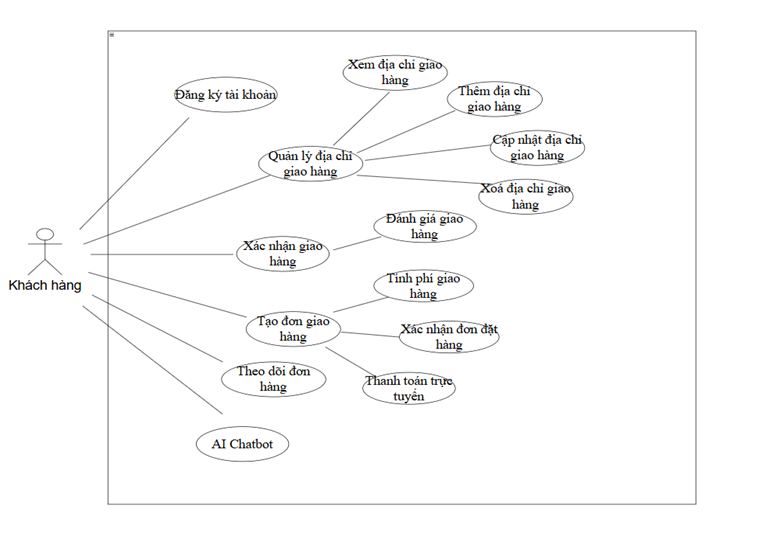
\includegraphics[width=6.5in,height=7.26597in,keepaspectratio,width=\linewidth]{images/Use case Diagram của Khách hàng.png}
\end{figure}

\textbf{Bảng mô tả các use case chính của Khách hàng}

\begin{longtable}{|L{3cm}|L{11cm}|}
\hline
\textbf{Thành phần} & \textbf{Nội dung} \\
\hline
\textbf{Use Case ID} & UC01 \\
\hline
\textbf{Tên Use Case} & Đăng ký tài khoản \\
\hline
\textbf{Actor chính} & Khách hàng \\
\hline
\textbf{Mô tả} & Cho phép khách hàng tạo tài khoản mới bằng email hoặc số điện thoại. \\
\hline
\textbf{Tiền điều kiện} & Khách hàng chưa có tài khoản trong hệ thống. \\
\hline
\textbf{Luồng chính} & \begin{itemize}[leftmargin=*,topsep=2pt,itemsep=2pt]
\item Khách hàng chọn Đăng ký
\item Nhập email/số điện thoại và thông tin tài khoản
\item Hệ thống kiểm tra tính hợp lệ của thông tin
\item Hệ thống xác minh thông tin đăng ký
\item Hệ thống tạo tài khoản mới
\item Thông báo đăng ký thành công
\end{itemize} \\
\hline
\textbf{Luồng rẽ nhánh} & \begin{itemize}[leftmargin=*,topsep=2pt,itemsep=2pt]
\item 3a: Thông tin không hợp lệ → hệ thống thông báo lỗi
\item 3b: Email/số điện thoại đã tồn tại → yêu cầu sử dụng thông tin khác
\item 4a: Xác minh thất bại → thông báo lỗi
\end{itemize} \\
\hline
\textbf{Hậu điều kiện} & Tài khoản khách hàng được tạo thành công. \\
\hline
\end{longtable}

\begin{longtable}{|C{3cm}|L{11cm}|}
\hline
\textbf{Thành phần} & \textbf{Nội dung} \\
\hline

\textbf{Use Case ID} & UC02 \\
\hline

\textbf{Tên Use Case} & Đăng nhập \\
\hline

\textbf{Actor chính} & Người dùng đã xác thực \\
\hline

\textbf{Mô tả} &
Cho phép người dùng đăng nhập vào hệ thống bằng thông tin đã đăng ký.
\\
\hline

\textbf{Tiền điều kiện} &
Tài khoản đã được đăng ký và đang hoạt động.
\\
\hline

\textbf{Luồng chính} &
\begin{itemize}[leftmargin=*,topsep=2pt,itemsep=2pt]
    \item 1. Người dùng nhập email/số điện thoại và mật khẩu.
    \item 2. Hệ thống kiểm tra thông tin đăng nhập.
    \item 3. Hệ thống xác thực tài khoản.
    \item 4. Hệ thống tạo phiên đăng nhập/JWT.
    \item 5. Chuyển người dùng đến giao diện phù hợp.
\end{itemize}
\\
\hline

\textbf{Luồng rẽ nhánh} &
\begin{itemize}[leftmargin=*,topsep=2pt,itemsep=2pt]
    \item 2a. Sai thông tin đăng nhập $\rightarrow$ thông báo lỗi.
    \item 3a. Tài khoản bị khóa $\rightarrow$ từ chối đăng nhập.
\end{itemize}
\\
\hline

\textbf{Hậu điều kiện} &
Người dùng đăng nhập thành công và được cấp quyền truy cập tương ứng.
\\
\hline

\end{longtable}

\begin{longtable}{|L{3cm}|L{11cm}|}
\hline
\textbf{Thành phần} & \textbf{Nội dung} \\
\hline
\textbf{Use Case ID} & UC14 \\
\hline
\textbf{Tên Use Case} & Tạo đơn giao hàng \\
\hline
\textbf{Actor chính} & Khách hàng \\
\hline
\textbf{Mô tả} & Cho phép khách hàng tạo yêu cầu giao hàng bằng Drone. \\
\hline
\textbf{Tiền điều kiện} & Khách hàng đã đăng nhập và có thông tin địa chỉ giao/nhận hợp lệ. \\
\hline
\textbf{Luồng chính} & \begin{itemize}[leftmargin=*,topsep=2pt,itemsep=2pt]
\item 1. Khách hàng chọn Tạo đơn giao hàng.
\item 2. Nhập/chọn địa chỉ nhận và giao hàng.
\item 3. Nhập thông tin kiện hàng.
\item 4. Hệ thống kiểm tra thông tin.
\item 5. Hệ thống tính phí giao hàng.
\item 6. Khách hàng kiểm tra thông tin đơn.
\item 7. Khách hàng xác nhận đơn.
\item 8. Hệ thống tạo đơn với trạng thái PENDING.
\end{itemize} \\
\hline
\textbf{Luồng rẽ nhánh} & \begin{itemize}[leftmargin=*,topsep=2pt,itemsep=2pt]
\item 4a. Thông tin không hợp lệ $\rightarrow$ thông báo lỗi và yêu cầu chỉnh sửa.
\item 5a. Không thể tính phí $\rightarrow$ thông báo lỗi.
\item 8a. Tạo đơn thất bại $\rightarrow$ thông báo lỗi.
\end{itemize} \\
\hline
\textbf{Hậu điều kiện} & Đơn giao hàng được tạo và chờ nhân viên điều phối xử lý. \\
\hline
\end{longtable}

\begin{longtable}{|L{3cm}|L{11cm}|}
\hline
\textbf{Thành phần} & \textbf{Nội dung} \\
\hline
\textbf{Use Case ID} & UC16 \\
\hline
\textbf{Tên Use Case} & Xác nhận đơn giao hàng \\
\hline
\textbf{Actor chính} & Khách hàng \\
\hline
\textbf{Mô tả} & Cho phép khách hàng kiểm tra và xác nhận thông tin trước khi gửi yêu cầu giao hàng. \\
\hline
\textbf{Tiền điều kiện} & Khách hàng đã nhập đầy đủ thông tin đơn hàng. \\
\hline
\textbf{Luồng chính} & \begin{itemize}[leftmargin=*,topsep=2pt,itemsep=2pt]
\item 1. Hệ thống hiển thị thông tin đơn hàng.
\item 2. Khách hàng kiểm tra địa chỉ, kiện hàng và phí giao hàng.
\item 3. Khách hàng chọn Xác nhận.
\item 4. Hệ thống kiểm tra lại dữ liệu.
\item 5. Hệ thống ghi nhận yêu cầu giao hàng.
\end{itemize} \\
\hline
\textbf{Luồng rẽ nhánh} & \begin{itemize}[leftmargin=*,topsep=2pt,itemsep=2pt]
\item 2a. Thông tin chưa chính xác $\rightarrow$ khách hàng chỉnh sửa đơn.
\item 4a. Dữ liệu không hợp lệ $\rightarrow$ hệ thống yêu cầu chỉnh sửa.
\end{itemize} \\
\hline
\textbf{Hậu điều kiện} & Yêu cầu giao hàng được xác nhận và chuyển sang trạng thái chờ xử lý. \\
\hline
\end{longtable}

\begin{longtable}{|L{3cm}|L{11cm}|}
\hline
\textbf{Thành phần} & \textbf{Nội dung} \\
\hline
\textbf{Use Case ID} & UC19 \\
\hline
\textbf{Tên Use Case} & Xem đơn hàng \\
\hline
\textbf{Actor chính} & Khách hàng \\
\hline
\textbf{Mô tả} & Cho phép khách hàng xem các đơn giao hàng hiện tại và lịch sử giao hàng. \\
\hline
\textbf{Tiền điều kiện} & Khách hàng đã đăng nhập. \\
\hline
\textbf{Luồng chính} & \begin{itemize}[leftmargin=*,topsep=2pt,itemsep=2pt]
\item 1. Khách hàng chọn Đơn hàng.
\item 2. Hệ thống lấy danh sách đơn hàng của khách hàng.
\item 3. Hệ thống hiển thị danh sách đơn hàng.
\item 4. Khách hàng chọn một đơn để xem chi tiết.
\end{itemize} \\
\hline
\textbf{Luồng rẽ nhánh} & \begin{itemize}[leftmargin=*,topsep=2pt,itemsep=2pt]
\item 2a. Không có đơn hàng $\rightarrow$ hệ thống thông báo chưa có đơn hàng.
\end{itemize} \\
\hline
\textbf{Hậu điều kiện} & Thông tin đơn hàng được hiển thị. \\
\hline
\end{longtable}

\begin{longtable}{|L{3cm}|L{11cm}|}
\hline
\textbf{Thành phần} & \textbf{Nội dung} \\
\hline
\textbf{Use Case ID} & UC20 \\
\hline
\textbf{Tên Use Case} & Chỉnh sửa đơn hàng \\
\hline
\textbf{Actor chính} & Khách hàng \\
\hline
\textbf{Mô tả} & Cho phép khách hàng thay đổi thông tin đơn hàng trước khi được phê duyệt. \\
\hline
\textbf{Tiền điều kiện} & Khách hàng đã đăng nhập và đơn hàng chưa được phê duyệt. \\
\hline
\textbf{Luồng chính} & \begin{itemize}[leftmargin=*,topsep=2pt,itemsep=2pt]
\item 1. Khách hàng chọn đơn hàng cần chỉnh sửa.
\item 2. Hệ thống kiểm tra trạng thái đơn.
\item 3. Khách hàng thay đổi thông tin.
\item 4. Hệ thống kiểm tra dữ liệu mới.
\item 5. Hệ thống cập nhật đơn hàng.
\item 6. Thông báo cập nhật thành công.
\end{itemize} \\
\hline
\textbf{Luồng rẽ nhánh} & \begin{itemize}[leftmargin=*,topsep=2pt,itemsep=2pt]
\item 2a. Đơn đã được phê duyệt $\rightarrow$ không cho phép chỉnh sửa.
\item 4a. Dữ liệu không hợp lệ $\rightarrow$ yêu cầu chỉnh sửa lại.
\end{itemize} \\
\hline
\textbf{Hậu điều kiện} & Thông tin đơn hàng được cập nhật. \\
\hline
\end{longtable}

\begin{longtable}{|L{3cm}|L{11cm}|}
\hline
\textbf{Thành phần} & \textbf{Nội dung} \\
\hline
\textbf{Use Case ID} & UC22 \\
\hline
\textbf{Tên Use Case} & Theo dõi giao hàng \\
\hline
\textbf{Actor chính} & Khách hàng \\
\hline
\textbf{Mô tả} & Cho phép khách hàng theo dõi trạng thái, vị trí Drone và ETA của đơn hàng. \\
\hline
\textbf{Tiền điều kiện} & Khách hàng đã đăng nhập và có đơn hàng đang được giao. \\
\hline
\textbf{Luồng chính} & \begin{itemize}[leftmargin=*,topsep=2pt,itemsep=2pt]
\item 1. Khách hàng chọn đơn hàng cần theo dõi.
\item 2. Hệ thống lấy trạng thái hiện tại của đơn.
\item 3. Hệ thống lấy vị trí Drone.
\item 4. Hệ thống lấy ETA dự kiến.
\item 5. Hệ thống hiển thị thông tin theo dõi.
\item 6. Hệ thống cập nhật thông tin khi trạng thái thay đổi.
\end{itemize} \\
\hline
\textbf{Luồng rẽ nhánh} & \begin{itemize}[leftmargin=*,topsep=2pt,itemsep=2pt]
\item 2a. Không nhận được dữ liệu Drone $\rightarrow$ hiển thị trạng thái gần nhất.
\item 4a. Không có ETA $\rightarrow$ thông báo ETA chưa khả dụng.
\end{itemize} \\
\hline
\textbf{Hậu điều kiện} & Khách hàng nhận được thông tin cập nhật về quá trình giao hàng. \\
\hline
\end{longtable}

\begin{longtable}{|L{3cm}|L{11cm}|}
\hline
\textbf{Thành phần} & \textbf{Nội dung} \\
\hline
\textbf{Use Case ID} & UC23 \\
\hline
\textbf{Tên Use Case} & Xác nhận giao hàng \\
\hline
\textbf{Actor chính} & Khách hàng \\
\hline
\textbf{Mô tả} & Cho phép khách hàng xác nhận đã nhận kiện hàng thành công. \\
\hline
\textbf{Tiền điều kiện} & Đơn hàng đã đến điểm giao và kiện hàng đã được giao đến khách hàng. \\
\hline
\textbf{Luồng chính} & \begin{itemize}[leftmargin=*,topsep=2pt,itemsep=2pt]
\item 1. Khách hàng nhận kiện hàng.
\item 2. Khách hàng mở thông tin đơn hàng.
\item 3. Chọn Xác nhận giao hàng.
\item 4. Hệ thống ghi nhận xác nhận.
\item 5. Hệ thống cập nhật trạng thái đơn thành DELIVERED.
\item 6. Hệ thống gửi thông báo hoàn tất.
\end{itemize} \\
\hline
\textbf{Luồng rẽ nhánh} & \begin{itemize}[leftmargin=*,topsep=2pt,itemsep=2pt]
\item 3a. Khách hàng không xác nhận $\rightarrow$ đơn hàng tiếp tục chờ xác nhận.
\item 4a. Xác nhận thất bại $\rightarrow$ hệ thống thông báo lỗi.
\end{itemize} \\
\hline
\textbf{Hậu điều kiện} & Đơn hàng được xác nhận hoàn tất. \\
\hline
\end{longtable}
\begin{longtable}{|L{3cm}|L{11cm}|}
\hline
\textbf{Thành phần} & \textbf{Nội dung} \\
\hline
\textbf{Use Case ID} & UC24 \\
\hline
\textbf{Tên Use Case} & Đánh giá giao hàng \\
\hline
\textbf{Actor chính} & Khách hàng \\
\hline
\textbf{Mô tả} & Cho phép khách hàng đánh giá chất lượng dịch vụ sau khi giao hàng hoàn tất. \\
\hline
\textbf{Tiền điều kiện} & Đơn hàng đã ở trạng thái DELIVERED. \\
\hline
\textbf{Luồng chính} & \begin{itemize}[leftmargin=*,topsep=2pt,itemsep=2pt]
\item 1. Khách hàng mở đơn hàng đã hoàn tất.
\item 2. Chọn chức năng đánh giá.
\item 3. Chọn mức đánh giá và nhập nhận xét.
\item 4. Gửi đánh giá.
\item 5. Hệ thống lưu đánh giá.
\end{itemize} \\
\hline
\textbf{Luồng rẽ nhánh} & \begin{itemize}[leftmargin=*,topsep=2pt,itemsep=2pt]
\item 3a. Nội dung đánh giá không hợp lệ $\rightarrow$ yêu cầu nhập lại.
\item 5a. Lưu thất bại $\rightarrow$ thông báo lỗi.
\end{itemize} \\
\hline
\textbf{Hậu điều kiện} & Đánh giá được lưu vào hệ thống. \\
\hline
\end{longtable}

\begin{longtable}{|L{3cm}|L{11cm}|}
\hline
\textbf{Thành phần} & \textbf{Nội dung} \\
\hline
\textbf{Use Case ID} & UC25 \\
\hline
\textbf{Tên Use Case} & Chatbot AI \\
\hline
\textbf{Actor chính} & Khách hàng \\
\hline
\textbf{Mô tả} & Cho phép khách hàng tương tác với Chatbot AI để được hỗ trợ về dịch vụ và đơn giao hàng. \\
\hline
\textbf{Tiền điều kiện} & Khách hàng đã đăng nhập và có quyền sử dụng Chatbot. \\
\hline
\textbf{Luồng chính} & \begin{itemize}[leftmargin=*,topsep=2pt,itemsep=2pt]
\item 1. Khách hàng mở Chatbot.
\item 2. Nhập câu hỏi hoặc yêu cầu hỗ trợ.
\item 3. Hệ thống gửi yêu cầu đến dịch vụ AI.
\item 4. AI phân tích nội dung.
\item 5. AI tạo câu trả lời.
\item 6. Hệ thống hiển thị câu trả lời cho khách hàng.
\end{itemize} \\
\hline
\textbf{Luồng rẽ nhánh} & \begin{itemize}[leftmargin=*,topsep=2pt,itemsep=2pt]
\item 3a. Dịch vụ AI không khả dụng $\rightarrow$ thông báo tạm thời không thể xử lý.
\item 4a. AI không hiểu yêu cầu $\rightarrow$ yêu cầu khách hàng diễn đạt lại.
\end{itemize} \\
\hline
\textbf{Hậu điều kiện} & Khách hàng nhận được phản hồi từ Chatbot AI. \\
\hline
\end{longtable}


% ==================================================================================================
% ==================================================================================================

\begin{itemize}
\item
  \textbf{Use case Diagram của Nhân viên điều phối} 
\end{itemize}

\begin{figure}[H]
\centering
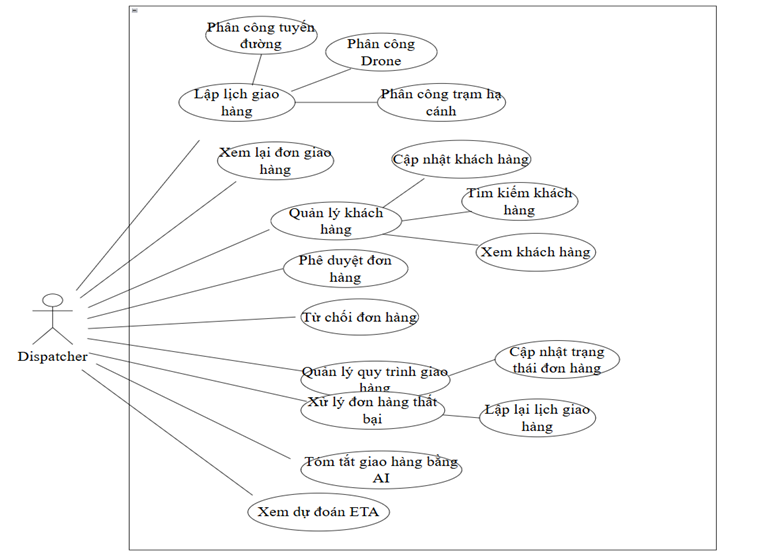
\includegraphics[width=6.5in,height=7.26597in,keepaspectratio,width=\linewidth]{images/Use case Diagram của Nhân viên điều phối.png}
\end{figure}

\textbf{Bảng mô tả các use case chính của Nhân viên điều phối}

\begin{longtable}{|C{3cm}|L{11cm}|}
\hline
\textbf{Thành phần} & \textbf{Nội dung} \\
\hline

\textbf{Use Case ID} & UC26 \\
\hline

\textbf{Tên Use Case} & Quản lý khách hàng \\
\hline

\textbf{Actor chính} & Nhân viên điều phối \\
\hline

\textbf{Mô tả} &
Cho phép nhân viên điều phối quản lý thông tin khách hàng phục vụ hoạt động giao hàng.
\\
\hline

\textbf{Tiền điều kiện} &
Nhân viên điều phối đã đăng nhập và có quyền quản lý khách hàng.
\\
\hline

\textbf{Luồng chính} &
\begin{itemize}[leftmargin=*,topsep=2pt,itemsep=2pt]
    \item 1. Nhân viên chọn chức năng quản lý khách hàng.
    \item 2. Hệ thống hiển thị danh sách khách hàng.
    \item 3. Nhân viên tìm kiếm hoặc chọn khách hàng.
    \item 4. Hệ thống hiển thị thông tin khách hàng.
    \item 5. Nhân viên thực hiện thao tác quản lý cần thiết.
    \item 6. Hệ thống lưu thay đổi.
\end{itemize}
\\
\hline

\textbf{Luồng rẽ nhánh} &
\begin{itemize}[leftmargin=*,topsep=2pt,itemsep=2pt]
    \item 3a. Không tìm thấy khách hàng $\rightarrow$ hệ thống thông báo không có kết quả.
    \item 6a. Dữ liệu không hợp lệ $\rightarrow$ hệ thống yêu cầu nhập lại.
\end{itemize}
\\
\hline

\textbf{Hậu điều kiện} &
Thông tin khách hàng được cập nhật hoặc hiển thị thành công.
\\
\hline

\end{longtable}

% ==================== UC31 ====================
\begin{longtable}{|C{3cm}|L{11cm}|}
\hline
\textbf{Thành phần} & \textbf{Nội dung} \\
\hline
\textbf{Use Case ID} & UC31 \\
\hline
\textbf{Tên Use Case} & Phê duyệt đơn hàng \\
\hline
\textbf{Actor chính} & Nhân viên điều phối \\
\hline
\textbf{Mô tả} &
Cho phép nhân viên điều phối phê duyệt yêu cầu giao hàng đủ điều kiện. \\
\hline
\textbf{Tiền điều kiện} &
Đơn hàng đang ở trạng thái chờ xử lý và thông tin hợp lệ. \\
\hline
\textbf{Luồng chính} &
\begin{itemize}[leftmargin=*,topsep=2pt,itemsep=2pt]
    \item 1. Nhân viên chọn đơn hàng cần phê duyệt.
    \item 2. Hệ thống kiểm tra thông tin đơn hàng.
    \item 3. Nhân viên chọn Phê duyệt.
    \item 4. Hệ thống cập nhật trạng thái đơn hàng thành APPROVED.
    \item 5. Hệ thống thông báo kết quả.
    \item 6. Đơn hàng được chuyển sang bước lập lịch giao hàng.
\end{itemize} \\
\hline
\textbf{Luồng rẽ nhánh} &
\begin{itemize}[leftmargin=*,topsep=2pt,itemsep=2pt]
    \item 2a. Đơn hàng không hợp lệ $\rightarrow$ không cho phép phê duyệt.
    \item 4a. Cập nhật thất bại $\rightarrow$ thông báo lỗi.
\end{itemize} \\
\hline
\textbf{Hậu điều kiện} &
Đơn hàng được phê duyệt và sẵn sàng lập lịch. \\
\hline
\end{longtable}


% ==================== UC32 ====================
\begin{longtable}{|C{3cm}|L{11cm}|}
\hline
\textbf{Thành phần} & \textbf{Nội dung} \\
\hline
\textbf{Use Case ID} & UC32 \\
\hline
\textbf{Tên Use Case} & Từ chối đơn hàng \\
\hline
\textbf{Actor chính} & Nhân viên điều phối \\
\hline
\textbf{Mô tả} &
Cho phép nhân viên điều phối từ chối các yêu cầu giao hàng không đáp ứng điều kiện. \\
\hline
\textbf{Tiền điều kiện} &
Đơn hàng đang chờ xử lý. \\
\hline
\textbf{Luồng chính} &
\begin{itemize}[leftmargin=*,topsep=2pt,itemsep=2pt]
    \item 1. Nhân viên chọn đơn hàng.
    \item 2. Kiểm tra thông tin và điều kiện giao hàng.
    \item 3. Chọn Từ chối.
    \item 4. Nhập lý do từ chối.
    \item 5. Hệ thống cập nhật trạng thái đơn hàng.
    \item 6. Hệ thống gửi thông báo cho khách hàng.
\end{itemize} \\
\hline
\textbf{Luồng rẽ nhánh} &
\begin{itemize}[leftmargin=*,topsep=2pt,itemsep=2pt]
    \item 4a. Không nhập lý do $\rightarrow$ yêu cầu bổ sung lý do.
    \item 5a. Cập nhật thất bại $\rightarrow$ thông báo lỗi.
\end{itemize} \\
\hline
\textbf{Hậu điều kiện} &
Đơn hàng bị từ chối và khách hàng nhận được thông báo. \\
\hline
\end{longtable}


% ==================== UC33 ====================
\begin{longtable}{|C{3cm}|L{11cm}|}
\hline
\textbf{Thành phần} & \textbf{Nội dung} \\
\hline
\textbf{Use Case ID} & UC33 \\
\hline
\textbf{Tên Use Case} & Lập lịch giao hàng \\
\hline
\textbf{Actor chính} & Nhân viên điều phối \\
\hline
\textbf{Mô tả} &
Cho phép nhân viên điều phối tạo lịch giao hàng cho các đơn đã được phê duyệt. \\
\hline
\textbf{Tiền điều kiện} &
Đơn hàng đã được phê duyệt. \\
\hline
\textbf{Luồng chính} &
\begin{itemize}[leftmargin=*,topsep=2pt,itemsep=2pt]
    \item 1. Nhân viên chọn đơn hàng đã phê duyệt.
    \item 2. Chọn thời gian giao hàng.
    \item 3. Hệ thống kiểm tra Drone và trạm khả dụng.
    \item 4. Nhân viên xác nhận lịch giao hàng.
    \item 5. Hệ thống lưu lịch giao hàng.
    \item 6. Hệ thống cập nhật trạng thái đơn hàng.
\end{itemize} \\
\hline
\textbf{Luồng rẽ nhánh} &
\begin{itemize}[leftmargin=*,topsep=2pt,itemsep=2pt]
    \item 3a. Không có Drone hoặc trạm phù hợp $\rightarrow$ thông báo và yêu cầu chọn thời gian khác.
    \item 5a. Lưu lịch thất bại $\rightarrow$ thông báo lỗi.
\end{itemize} \\
\hline
\textbf{Hậu điều kiện} &
Đơn hàng có lịch giao hàng và sẵn sàng được phân công. \\
\hline
\end{longtable}


% ==================== UC34 ====================
\begin{longtable}{|C{3cm}|L{11cm}|}
\hline
\textbf{Thành phần} & \textbf{Nội dung} \\
\hline
\textbf{Use Case ID} & UC34 \\
\hline
\textbf{Tên Use Case} & Phân công Drone \\
\hline
\textbf{Actor chính} & Nhân viên điều phối \\
\hline
\textbf{Mô tả} &
Cho phép nhân viên điều phối lựa chọn Drone phù hợp để thực hiện đơn giao hàng. \\
\hline
\textbf{Tiền điều kiện} &
Đơn hàng đã được phê duyệt và có lịch giao hàng. \\
\hline
\textbf{Luồng chính} &
\begin{itemize}[leftmargin=*,topsep=2pt,itemsep=2pt]
    \item 1. Nhân viên chọn đơn hàng cần phân công.
    \item 2. Hệ thống tìm các Drone khả dụng.
    \item 3. Hệ thống kiểm tra tải trọng và trạng thái Drone.
    \item 4. Hiển thị danh sách Drone phù hợp.
    \item 5. Nhân viên chọn Drone.
    \item 6. Hệ thống lưu thông tin phân công.
    \item 7. Cập nhật trạng thái Drone và đơn hàng.
\end{itemize} \\
\hline
\textbf{Luồng rẽ nhánh} &
\begin{itemize}[leftmargin=*,topsep=2pt,itemsep=2pt]
    \item 2a. Không có Drone khả dụng $\rightarrow$ thông báo chưa thể phân công.
    \item 3a. Drone không đáp ứng tải trọng $\rightarrow$ loại khỏi danh sách.
    \item 6a. Phân công thất bại $\rightarrow$ thông báo lỗi.
\end{itemize} \\
\hline
\textbf{Hậu điều kiện} &
Drone được phân công cho đơn giao hàng. \\
\hline
\end{longtable}


% ==================== UC35 ====================
\begin{longtable}{|C{3cm}|L{11cm}|}
\hline
\textbf{Thành phần} & \textbf{Nội dung} \\
\hline
\textbf{Use Case ID} & UC35 \\
\hline
\textbf{Tên Use Case} & Phân công trạm hạ cánh \\
\hline
\textbf{Actor chính} & Nhân viên điều phối \\
\hline
\textbf{Mô tả} &
Lựa chọn trạm hạ cánh phù hợp cho quá trình tiếp nhận và giao nhận kiện hàng. \\
\hline
\textbf{Tiền điều kiện} &
Đơn hàng đã được phê duyệt. \\
\hline
\textbf{Luồng chính} &
\begin{itemize}[leftmargin=*,topsep=2pt,itemsep=2pt]
    \item 1. Nhân viên chọn đơn hàng.
    \item 2. Hệ thống tìm các trạm phù hợp.
    \item 3. Kiểm tra vị trí và sức chứa trạm.
    \item 4. Nhân viên chọn trạm xuất phát và trạm đến.
    \item 5. Hệ thống lưu thông tin trạm.
\end{itemize} \\
\hline
\textbf{Luồng rẽ nhánh} &
\begin{itemize}[leftmargin=*,topsep=2pt,itemsep=2pt]
    \item 2a. Không có trạm phù hợp $\rightarrow$ thông báo lỗi.
    \item 3a. Trạm hết sức chứa $\rightarrow$ loại trạm khỏi danh sách.
\end{itemize} \\
\hline
\textbf{Hậu điều kiện} &
Trạm xuất phát và trạm đến được xác định cho đơn hàng. \\
\hline
\end{longtable}


% ==================== UC36 ====================
\begin{longtable}{|C{3cm}|L{11cm}|}
\hline
\textbf{Thành phần} & \textbf{Nội dung} \\
\hline
\textbf{Use Case ID} & UC36 \\
\hline
\textbf{Tên Use Case} & Phân công tuyến đường \\
\hline
\textbf{Actor chính} & Nhân viên điều phối \\
\hline
\textbf{Mô tả} &
Xác định tuyến đường phù hợp để Drone thực hiện giao hàng. \\
\hline
\textbf{Tiền điều kiện} &
Drone và các trạm đã được xác định. \\
\hline
\textbf{Luồng chính} &
\begin{itemize}[leftmargin=*,topsep=2pt,itemsep=2pt]
    \item 1. Nhân viên chọn đơn giao hàng.
    \item 2. Hệ thống lấy vị trí điểm đi và điểm đến.
    \item 3. Hệ thống xác định tuyến đường phù hợp.
    \item 4. Nhân viên kiểm tra tuyến đường.
    \item 5. Xác nhận tuyến đường.
    \item 6. Hệ thống lưu tuyến đường giao hàng.
\end{itemize} \\
\hline
\textbf{Luồng rẽ nhánh} &
\begin{itemize}[leftmargin=*,topsep=2pt,itemsep=2pt]
    \item 3a. Không xác định được tuyến đường $\rightarrow$ thông báo lỗi.
    \item 4a. Tuyến đường không phù hợp $\rightarrow$ chọn tuyến khác.
\end{itemize} \\
\hline
\textbf{Hậu điều kiện} &
Tuyến đường giao hàng được lưu cho chuyến giao. \\
\hline
\end{longtable}


% ==================== UC37 ====================
\begin{longtable}{|C{3cm}|L{11cm}|}
\hline
\textbf{Thành phần} & \textbf{Nội dung} \\
\hline
\textbf{Use Case ID} & UC37 \\
\hline
\textbf{Tên Use Case} & Quản lý quy trình giao hàng \\
\hline
\textbf{Actor chính} & Nhân viên điều phối \\
\hline
\textbf{Mô tả} &
Theo dõi và quản lý đơn hàng trong toàn bộ vòng đời giao hàng. \\
\hline
\textbf{Tiền điều kiện} &
Nhân viên đã đăng nhập và có quyền điều phối. \\
\hline
\textbf{Luồng chính} &
\begin{itemize}[leftmargin=*,topsep=2pt,itemsep=2pt]
    \item 1. Nhân viên mở danh sách chuyến giao.
    \item 2. Hệ thống hiển thị trạng thái các đơn hàng.
    \item 3. Nhân viên theo dõi tiến trình giao hàng.
    \item 4. Xử lý các vấn đề phát sinh nếu có.
    \item 5. Hệ thống cập nhật trạng thái tương ứng.
\end{itemize} \\
\hline
\textbf{Luồng rẽ nhánh} &
\begin{itemize}[leftmargin=*,topsep=2pt,itemsep=2pt]
    \item 4a. Giao hàng thất bại $\rightarrow$ chuyển sang UC39 -- Xử lý giao hàng thất bại.
\end{itemize} \\
\hline
\textbf{Hậu điều kiện} &
Trạng thái và tiến trình giao hàng được cập nhật. \\
\hline
\end{longtable}


% ==================== UC38 ====================
\begin{longtable}{|C{3cm}|L{11cm}|}
\hline
\textbf{Thành phần} & \textbf{Nội dung} \\
\hline
\textbf{Use Case ID} & UC38 \\
\hline
\textbf{Tên Use Case} & Cập nhật trạng thái đơn hàng \\
\hline
\textbf{Actor chính} & Nhân viên điều phối \\
\hline
\textbf{Mô tả} &
Cho phép nhân viên cập nhật trạng thái đơn hàng trong quá trình xử lý. \\
\hline
\textbf{Tiền điều kiện} &
Đơn hàng tồn tại và nhân viên có quyền cập nhật. \\
\hline
\textbf{Luồng chính} &
\begin{itemize}[leftmargin=*,topsep=2pt,itemsep=2pt]
    \item 1. Nhân viên chọn đơn hàng.
    \item 2. Chọn trạng thái mới.
    \item 3. Hệ thống kiểm tra trạng thái hợp lệ.
    \item 4. Lưu trạng thái mới.
    \item 5. Gửi thông báo đến các bên liên quan.
\end{itemize} \\
\hline
\textbf{Luồng rẽ nhánh} &
\begin{itemize}[leftmargin=*,topsep=2pt,itemsep=2pt]
    \item 3a. Trạng thái không hợp lệ $\rightarrow$ từ chối cập nhật.
    \item 4a. Lưu thất bại $\rightarrow$ thông báo lỗi.
\end{itemize} \\
\hline
\textbf{Hậu điều kiện} &
Trạng thái đơn hàng được cập nhật. \\
\hline
\end{longtable}


% ==================== UC39 ====================
\begin{longtable}{|C{3cm}|L{11cm}|}
\hline
\textbf{Thành phần} & \textbf{Nội dung} \\
\hline
\textbf{Use Case ID} & UC39 \\
\hline
\textbf{Tên Use Case} & Xử lý giao hàng thất bại \\
\hline
\textbf{Actor chính} & Nhân viên điều phối \\
\hline
\textbf{Mô tả} &
Cho phép xử lý các trường hợp giao hàng thất bại và quyết định phương án tiếp theo. \\
\hline
\textbf{Tiền điều kiện} &
Chuyến giao hàng được ghi nhận ở trạng thái thất bại. \\
\hline
\textbf{Luồng chính} &
\begin{itemize}[leftmargin=*,topsep=2pt,itemsep=2pt]
    \item 1. Hệ thống ghi nhận giao hàng thất bại.
    \item 2. Nhân viên xem thông tin và nguyên nhân thất bại.
    \item 3. Đánh giá tình trạng đơn hàng.
    \item 4. Chọn phương án lập lại lịch giao hoặc hoàn trả/hủy đơn.
    \item 5. Hệ thống cập nhật thông tin xử lý.
    \item 6. Gửi thông báo cho khách hàng.
\end{itemize} \\
\hline
\textbf{Luồng rẽ nhánh} &
\begin{itemize}[leftmargin=*,topsep=2pt,itemsep=2pt]
    \item 4a. Chọn giao lại $\rightarrow$ chuyển sang UC40 -- Lập lại lịch giao hàng.
    \item 4b. Không thể giao lại $\rightarrow$ thực hiện hoàn trả/hủy đơn.
    \item 5a. Cập nhật thất bại $\rightarrow$ thông báo lỗi.
\end{itemize} \\
\hline
\textbf{Hậu điều kiện} &
Đơn hàng được lập lịch giao lại hoặc chuyển sang trạng thái xử lý cuối cùng. \\
\hline
\end{longtable}


% ==================== UC40 ====================
\begin{longtable}{|C{3cm}|L{11cm}|}
\hline
\textbf{Thành phần} & \textbf{Nội dung} \\
\hline
\textbf{Use Case ID} & UC40 \\
\hline
\textbf{Tên Use Case} & Lập lại lịch giao hàng \\
\hline
\textbf{Actor chính} & Nhân viên điều phối \\
\hline
\textbf{Mô tả} &
Tạo lịch giao hàng mới cho đơn hàng bị giao thất bại. \\
\hline
\textbf{Tiền điều kiện} &
Đơn hàng được xác định là có thể giao lại. \\
\hline
\textbf{Luồng chính} &
\begin{itemize}[leftmargin=*,topsep=2pt,itemsep=2pt]
    \item 1. Nhân viên chọn đơn hàng thất bại.
    \item 2. Chọn thời gian giao lại.
    \item 3. Hệ thống kiểm tra Drone và trạm khả dụng.
    \item 4. Chọn Drone và trạm phù hợp.
    \item 5. Nhân viên xác nhận lịch mới.
    \item 6. Hệ thống lưu lịch giao lại.
    \item 7. Gửi thông báo cho khách hàng.
\end{itemize} \\
\hline
\textbf{Luồng rẽ nhánh} &
\begin{itemize}[leftmargin=*,topsep=2pt,itemsep=2pt]
    \item 3a. Không có tài nguyên phù hợp $\rightarrow$ yêu cầu chọn thời gian khác.
    \item 6a. Lập lịch thất bại $\rightarrow$ thông báo lỗi.
\end{itemize} \\
\hline
\textbf{Hậu điều kiện} &
Đơn hàng có lịch giao mới và sẵn sàng thực hiện lại. \\
\hline
\end{longtable}


% ==================== UC41 ====================
\begin{longtable}{|C{3cm}|L{11cm}|}
\hline
\textbf{Thành phần} & \textbf{Nội dung} \\
\hline
\textbf{Use Case ID} & UC41 \\
\hline
\textbf{Tên Use Case} & Tóm tắt giao hàng bằng AI \\
\hline
\textbf{Actor chính} & Nhân viên điều phối \\
\hline
\textbf{Mô tả} &
Cho phép nhân viên xem bản tóm tắt và đề xuất về hoạt động giao hàng do AI tạo ra. \\
\hline
\textbf{Tiền điều kiện} &
Có dữ liệu giao hàng trong hệ thống. \\
\hline
\textbf{Luồng chính} &
\begin{itemize}[leftmargin=*,topsep=2pt,itemsep=2pt]
    \item 1. Nhân viên chọn chức năng tóm tắt AI.
    \item 2. Hệ thống lấy dữ liệu giao hàng.
    \item 3. Gửi dữ liệu đến dịch vụ AI.
    \item 4. AI phân tích dữ liệu.
    \item 5. AI tạo bản tóm tắt.
    \item 6. Hệ thống hiển thị kết quả.
\end{itemize} \\
\hline
\textbf{Luồng rẽ nhánh} &
\begin{itemize}[leftmargin=*,topsep=2pt,itemsep=2pt]
    \item 3a. Dịch vụ AI không khả dụng $\rightarrow$ thông báo lỗi.
    \item 4a. Không đủ dữ liệu $\rightarrow$ không thể tạo tóm tắt.
\end{itemize} \\
\hline
\textbf{Hậu điều kiện} &
Bản tóm tắt giao hàng được hiển thị. \\
\hline
\end{longtable}


% ==================== UC42 ====================
\begin{longtable}{|C{3cm}|L{11cm}|}
\hline
\textbf{Thành phần} & \textbf{Nội dung} \\
\hline
\textbf{Use Case ID} & UC42 \\
\hline
\textbf{Tên Use Case} & Xem dự đoán ETA \\
\hline
\textbf{Actor chính} & Nhân viên điều phối \\
\hline
\textbf{Mô tả} &
Cho phép nhân viên xem thời gian đến dự kiến của Drone do hệ thống AI dự đoán. \\
\hline
\textbf{Tiền điều kiện} &
Đơn hàng đang được thực hiện và có dữ liệu vị trí Drone. \\
\hline
\textbf{Luồng chính} &
\begin{itemize}[leftmargin=*,topsep=2pt,itemsep=2pt]
    \item 1. Nhân viên chọn đơn hàng đang giao.
    \item 2. Hệ thống lấy vị trí Drone và thông tin chuyến giao.
    \item 3. Gửi dữ liệu đến dịch vụ AI.
    \item 4. AI tính toán ETA.
    \item 5. Hệ thống nhận kết quả.
    \item 6. Hiển thị ETA cho nhân viên.
\end{itemize} \\
\hline
\textbf{Luồng rẽ nhánh} &
\begin{itemize}[leftmargin=*,topsep=2pt,itemsep=2pt]
    \item 2a. Không có dữ liệu vị trí $\rightarrow$ thông báo chưa thể dự đoán ETA.
    \item 4a. AI không trả kết quả $\rightarrow$ sử dụng ETA gần nhất hoặc thông báo lỗi.
\end{itemize} \\
\hline
\textbf{Hậu điều kiện} &
ETA dự kiến của chuyến giao được hiển thị và có thể được cập nhật vào đơn hàng. \\
\hline
\end{longtable}

% ==================================================================================================
% ==================================================================================================

\begin{itemize}
\item
  \textbf{Use case Diagram của Nhân viên vận hành trạm} 
\end{itemize}

\begin{figure}[H]
\centering
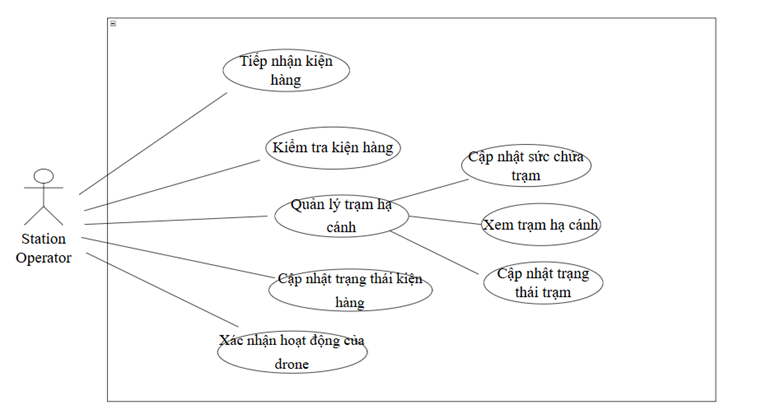
\includegraphics[width=6.5in,height=7.26597in,keepaspectratio,width=\linewidth]{images/Use case Diagram của Nhân viên vận hành trạm.png}
\end{figure}

\textbf{Bảng mô tả các use case chính của Nhân viên vận hành trạm}

% ==================== UC43 ====================
\begin{longtable}{|C{3cm}|L{11cm}|}
\hline
\textbf{Thành phần} & \textbf{Nội dung} \\
\hline
\textbf{Use Case ID} & UC43 \\
\hline
\textbf{Tên Use Case} & Tiếp nhận kiện hàng \\
\hline
\textbf{Actor chính} & Nhân viên vận hành trạm \\
\hline
\textbf{Mô tả} &
Cho phép nhân viên tiếp nhận kiện hàng tại trạm hạ cánh để chuẩn bị cho quá trình giao hàng.
\\
\hline
\textbf{Tiền điều kiện} &
Nhân viên đã đăng nhập và trạm đang hoạt động.
\\
\hline
\textbf{Luồng chính} &
\begin{itemize}[leftmargin=*,topsep=2pt,itemsep=2pt]
    \item 1. Nhân viên chọn chức năng tiếp nhận kiện hàng.
    \item 2. Quét hoặc nhập mã kiện hàng.
    \item 3. Hệ thống kiểm tra thông tin kiện hàng.
    \item 4. Nhân viên tiếp nhận kiện hàng.
    \item 5. Hệ thống ghi nhận kiện hàng tại trạm.
    \item 6. Cập nhật trạng thái kiện hàng.
\end{itemize}
\\
\hline
\textbf{Luồng rẽ nhánh} &
\begin{itemize}[leftmargin=*,topsep=2pt,itemsep=2pt]
    \item 3a. Không tìm thấy kiện hàng $\rightarrow$ thông báo lỗi.
    \item 3b. Kiện hàng không thuộc lịch giao $\rightarrow$ từ chối tiếp nhận.
    \item 5a. Lưu thông tin thất bại $\rightarrow$ thông báo lỗi.
\end{itemize}
\\
\hline
\textbf{Hậu điều kiện} &
Kiện hàng được ghi nhận đã tiếp nhận tại trạm.
\\
\hline
\end{longtable}


% ==================== UC44 ====================
\begin{longtable}{|C{3cm}|L{11cm}|}
\hline
\textbf{Thành phần} & \textbf{Nội dung} \\
\hline
\textbf{Use Case ID} & UC44 \\
\hline
\textbf{Tên Use Case} & Kiểm tra kiện hàng \\
\hline
\textbf{Actor chính} & Nhân viên vận hành trạm \\
\hline
\textbf{Mô tả} &
Kiểm tra trọng lượng, kích thước, tình trạng và thông tin của kiện hàng trước khi vận chuyển.
\\
\hline
\textbf{Tiền điều kiện} &
Kiện hàng đã được tiếp nhận tại trạm.
\\
\hline
\textbf{Luồng chính} &
\begin{itemize}[leftmargin=*,topsep=2pt,itemsep=2pt]
    \item 1. Nhân viên chọn kiện hàng cần kiểm tra.
    \item 2. Kiểm tra mã kiện hàng.
    \item 3. Kiểm tra trọng lượng và kích thước.
    \item 4. Kiểm tra tình trạng kiện hàng.
    \item 5. Đối chiếu với thông tin đơn hàng.
    \item 6. Hệ thống ghi nhận kết quả kiểm tra.
\end{itemize}
\\
\hline
\textbf{Luồng rẽ nhánh} &
\begin{itemize}[leftmargin=*,topsep=2pt,itemsep=2pt]
    \item 3a. Trọng lượng vượt giới hạn $\rightarrow$ đánh dấu không hợp lệ.
    \item 4a. Kiện hàng bị hư hỏng $\rightarrow$ ghi nhận sự cố.
    \item 5a. Thông tin không khớp $\rightarrow$ yêu cầu kiểm tra lại.
\end{itemize}
\\
\hline
\textbf{Hậu điều kiện} &
Kết quả kiểm tra kiện hàng được lưu vào hệ thống.
\\
\hline
\end{longtable}


% ==================== UC45 ====================
\begin{longtable}{|C{3cm}|L{11cm}|}
\hline
\textbf{Thành phần} & \textbf{Nội dung} \\
\hline
\textbf{Use Case ID} & UC45 \\
\hline
\textbf{Tên Use Case} & Quản lý trạm hạ cánh \\
\hline
\textbf{Actor chính} & Nhân viên vận hành trạm \\
\hline
\textbf{Mô tả} &
Cho phép nhân viên theo dõi và quản lý trạng thái hoạt động, sức chứa và tình trạng của trạm.
\\
\hline
\textbf{Tiền điều kiện} &
Nhân viên đã đăng nhập và được phân quyền quản lý trạm.
\\
\hline
\textbf{Luồng chính} &
\begin{itemize}[leftmargin=*,topsep=2pt,itemsep=2pt]
    \item 1. Nhân viên mở thông tin trạm.
    \item 2. Hệ thống hiển thị trạng thái và sức chứa.
    \item 3. Nhân viên kiểm tra tình trạng trạm.
    \item 4. Thực hiện cập nhật khi cần thiết.
    \item 5. Hệ thống lưu thông tin thay đổi.
\end{itemize}
\\
\hline
\textbf{Luồng rẽ nhánh} &
\begin{itemize}[leftmargin=*,topsep=2pt,itemsep=2pt]
    \item 4a. Không có quyền cập nhật $\rightarrow$ hệ thống từ chối thao tác.
    \item 5a. Cập nhật thất bại $\rightarrow$ thông báo lỗi.
\end{itemize}
\\
\hline
\textbf{Hậu điều kiện} &
Thông tin trạm được cập nhật chính xác.
\\
\hline
\end{longtable}


% ==================== UC46 ====================
\begin{longtable}{|C{3cm}|L{11cm}|}
\hline
\textbf{Thành phần} & \textbf{Nội dung} \\
\hline
\textbf{Use Case ID} & UC46 \\
\hline
\textbf{Tên Use Case} & Xem trạm hạ cánh \\
\hline
\textbf{Actor chính} & Nhân viên vận hành trạm \\
\hline
\textbf{Mô tả} &
Cho phép nhân viên xem thông tin và trạng thái hiện tại của trạm hạ cánh.
\\
\hline
\textbf{Tiền điều kiện} &
Nhân viên đã đăng nhập.
\\
\hline
\textbf{Luồng chính} &
\begin{itemize}[leftmargin=*,topsep=2pt,itemsep=2pt]
    \item 1. Nhân viên chọn chức năng xem trạm.
    \item 2. Hệ thống truy vấn thông tin trạm.
    \item 3. Hệ thống hiển thị trạng thái hoạt động, sức chứa và thông tin liên quan.
\end{itemize}
\\
\hline
\textbf{Luồng rẽ nhánh} &
\begin{itemize}[leftmargin=*,topsep=2pt,itemsep=2pt]
    \item 2a. Không thể lấy dữ liệu $\rightarrow$ hệ thống thông báo lỗi.
\end{itemize}
\\
\hline
\textbf{Hậu điều kiện} &
Thông tin trạm được hiển thị.
\\
\hline
\end{longtable}


% ==================== UC47 ====================
\begin{longtable}{|C{3cm}|L{11cm}|}
\hline
\textbf{Thành phần} & \textbf{Nội dung} \\
\hline
\textbf{Use Case ID} & UC47 \\
\hline
\textbf{Tên Use Case} & Cập nhật trạng thái trạm \\
\hline
\textbf{Actor chính} & Nhân viên vận hành trạm \\
\hline
\textbf{Mô tả} &
Cho phép nhân viên cập nhật trạng thái hoạt động của trạm.
\\
\hline
\textbf{Tiền điều kiện} &
Nhân viên đã đăng nhập và có quyền cập nhật trạm.
\\
\hline
\textbf{Luồng chính} &
\begin{itemize}[leftmargin=*,topsep=2pt,itemsep=2pt]
    \item 1. Nhân viên mở thông tin trạm.
    \item 2. Chọn trạng thái mới.
    \item 3. Hệ thống kiểm tra trạng thái hợp lệ.
    \item 4. Nhân viên xác nhận cập nhật.
    \item 5. Hệ thống lưu trạng thái mới.
\end{itemize}
\\
\hline
\textbf{Luồng rẽ nhánh} &
\begin{itemize}[leftmargin=*,topsep=2pt,itemsep=2pt]
    \item 3a. Trạng thái không hợp lệ $\rightarrow$ yêu cầu chọn lại.
    \item 5a. Cập nhật thất bại $\rightarrow$ thông báo lỗi.
\end{itemize}
\\
\hline
\textbf{Hậu điều kiện} &
Trạng thái trạm được cập nhật.
\\
\hline
\end{longtable}


% ==================== UC48 ====================
\begin{longtable}{|C{3cm}|L{11cm}|}
\hline
\textbf{Thành phần} & \textbf{Nội dung} \\
\hline
\textbf{Use Case ID} & UC48 \\
\hline
\textbf{Tên Use Case} & Cập nhật sức chứa trạm \\
\hline
\textbf{Actor chính} & Nhân viên vận hành trạm \\
\hline
\textbf{Mô tả} &
Cho phép nhân viên cập nhật số lượng kiện hàng hoặc vị trí còn khả dụng tại trạm.
\\
\hline
\textbf{Tiền điều kiện} &
Trạm đang hoạt động và nhân viên có quyền cập nhật.
\\
\hline
\textbf{Luồng chính} &
\begin{itemize}[leftmargin=*,topsep=2pt,itemsep=2pt]
    \item 1. Nhân viên mở thông tin sức chứa.
    \item 2. Nhập hoặc cập nhật số lượng hiện tại.
    \item 3. Hệ thống kiểm tra dữ liệu.
    \item 4. Lưu thông tin sức chứa mới.
    \item 5. Hiển thị kết quả cập nhật.
\end{itemize}
\\
\hline
\textbf{Luồng rẽ nhánh} &
\begin{itemize}[leftmargin=*,topsep=2pt,itemsep=2pt]
    \item 3a. Số liệu không hợp lệ $\rightarrow$ yêu cầu nhập lại.
    \item 4a. Sức chứa vượt giới hạn $\rightarrow$ từ chối cập nhật.
\end{itemize}
\\
\hline
\textbf{Hậu điều kiện} &
Sức chứa khả dụng của trạm được cập nhật.
\\
\hline
\end{longtable}


% ==================== UC49 ====================
\begin{longtable}{|C{3cm}|L{11cm}|}
\hline
\textbf{Thành phần} & \textbf{Nội dung} \\
\hline
\textbf{Use Case ID} & UC49 \\
\hline
\textbf{Tên Use Case} & Cập nhật trạng thái kiện hàng \\
\hline
\textbf{Actor chính} & Nhân viên vận hành trạm \\
\hline
\textbf{Mô tả} &
Cho phép nhân viên cập nhật trạng thái kiện hàng trong quá trình tiếp nhận và giao nhận tại trạm.
\\
\hline
\textbf{Tiền điều kiện} &
Kiện hàng đã được ghi nhận trong hệ thống.
\\
\hline
\textbf{Luồng chính} &
\begin{itemize}[leftmargin=*,topsep=2pt,itemsep=2pt]
    \item 1. Nhân viên chọn kiện hàng.
    \item 2. Kiểm tra trạng thái hiện tại.
    \item 3. Chọn trạng thái mới.
    \item 4. Hệ thống kiểm tra tính hợp lệ của trạng thái.
    \item 5. Lưu trạng thái mới.
    \item 6. Hệ thống thông báo cập nhật thành công.
\end{itemize}
\\
\hline
\textbf{Luồng rẽ nhánh} &
\begin{itemize}[leftmargin=*,topsep=2pt,itemsep=2pt]
    \item 4a. Trạng thái không phù hợp với quy trình $\rightarrow$ từ chối cập nhật.
    \item 5a. Lưu thất bại $\rightarrow$ thông báo lỗi.
\end{itemize}
\\
\hline
\textbf{Hậu điều kiện} &
Trạng thái kiện hàng được cập nhật và sẵn sàng cho bước tiếp theo.
\\
\hline
\end{longtable}


% ==================== UC50 ====================
\begin{longtable}{|C{3cm}|L{11cm}|}
\hline
\textbf{Thành phần} & \textbf{Nội dung} \\
\hline
\textbf{Use Case ID} & UC50 \\
\hline
\textbf{Tên Use Case} & Xác nhận hoạt động của Drone \\
\hline
\textbf{Actor chính} & Nhân viên vận hành trạm \\
\hline
\textbf{Mô tả} &
Cho phép nhân viên kiểm tra và xác nhận Drone đã được chuẩn bị, xếp kiện hàng và sẵn sàng cất cánh.
\\
\hline
\textbf{Tiền điều kiện} &
Drone đã được phân công và kiện hàng đã được tiếp nhận, kiểm tra.
\\
\hline
\textbf{Luồng chính} &
\begin{itemize}[leftmargin=*,topsep=2pt,itemsep=2pt]
    \item 1. Nhân viên chọn Drone được phân công.
    \item 2. Kiểm tra tình trạng Drone.
    \item 3. Kiểm tra pin và khả năng tải.
    \item 4. Kiểm tra kiện hàng đã được xếp đúng vị trí.
    \item 5. Nhân viên xác nhận Drone sẵn sàng.
    \item 6. Hệ thống cập nhật trạng thái Drone thành IN\_FLIGHT/READY theo quy trình.
    \item 7. Hệ thống ghi nhận thời điểm xác nhận.
\end{itemize}
\\
\hline
\textbf{Luồng rẽ nhánh} &
\begin{itemize}[leftmargin=*,topsep=2pt,itemsep=2pt]
    \item 2a. Drone gặp lỗi $\rightarrow$ không cho phép xuất phát.
    \item 3a. Pin không đủ $\rightarrow$ yêu cầu sạc Drone.
    \item 4a. Kiện hàng không đạt yêu cầu $\rightarrow$ yêu cầu kiểm tra lại.
    \item 5a. Nhân viên không xác nhận $\rightarrow$ giữ nguyên trạng thái.
\end{itemize}
\\
\hline
\textbf{Hậu điều kiện} &
Drone được xác nhận sẵn sàng cho chuyến giao hàng hoặc được chuyển sang trạng thái xử lý sự cố.
\\
\hline
\end{longtable}


% ==================================================================================================
% ==================================================================================================


\begin{itemize}
\item
  \textbf{Use case Diagram của Quản lý logitic} 
\end{itemize}

\begin{figure}[H]
\centering
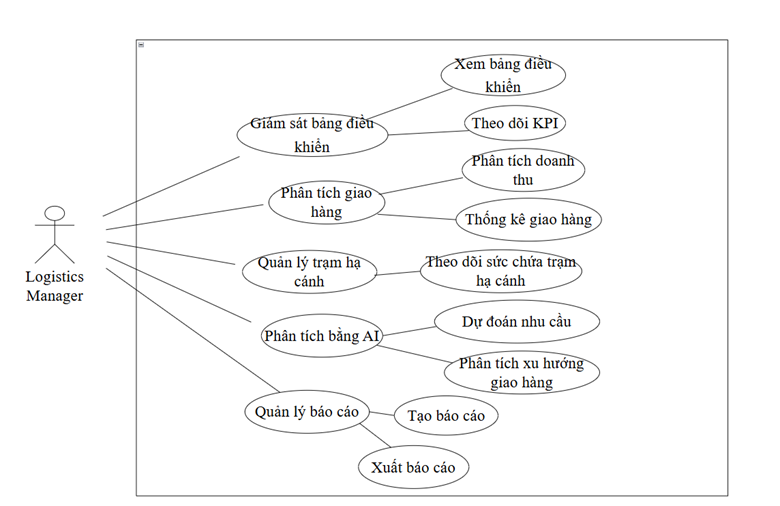
\includegraphics[width=6.5in,height=7.26597in,keepaspectratio,width=\linewidth]{images/Use case Diagram của Quản lý logistic.png}
\end{figure}

\textbf{Bảng mô tả các use case chính của Quản lý logistic}

% =========================================================
% UC43 - Tiếp nhận kiện hàng
% =========================================================
\begin{longtable}{|C{3cm}|L{11cm}|}
\hline
\textbf{Thành phần} & \textbf{Nội dung} \\
\hline
\textbf{Use Case ID} & UC43 \\
\hline
\textbf{Tên Use Case} & Tiếp nhận kiện hàng \\
\hline
\textbf{Actor chính} & Nhân viên vận hành trạm \\
\hline
\textbf{Mô tả} & Cho phép nhân viên tiếp nhận kiện hàng tại trạm hạ cánh để chuẩn bị cho quá trình giao hàng. \\
\hline
\textbf{Tiền điều kiện} & Nhân viên đã đăng nhập và trạm đang hoạt động. \\
\hline
\textbf{Luồng chính} &
\begin{itemize}[leftmargin=*,topsep=2pt,itemsep=2pt]
    \item 1. Nhân viên chọn chức năng tiếp nhận kiện hàng.
    \item 2. Quét hoặc nhập mã kiện hàng.
    \item 3. Hệ thống kiểm tra thông tin kiện hàng.
    \item 4. Nhân viên tiếp nhận kiện hàng.
    \item 5. Hệ thống ghi nhận kiện hàng tại trạm.
    \item 6. Cập nhật trạng thái kiện hàng.
\end{itemize} \\
\hline
\textbf{Luồng rẽ nhánh} &
\begin{itemize}[leftmargin=*,topsep=2pt,itemsep=2pt]
    \item 3a. Không tìm thấy kiện hàng $\rightarrow$ thông báo lỗi.
    \item 3b. Kiện hàng không thuộc lịch giao $\rightarrow$ từ chối tiếp nhận.
    \item 5a. Lưu thông tin thất bại $\rightarrow$ thông báo lỗi.
\end{itemize} \\
\hline
\textbf{Hậu điều kiện} & Kiện hàng được ghi nhận đã tiếp nhận tại trạm. \\
\hline
\end{longtable}


% =========================================================
% UC44 - Kiểm tra kiện hàng
% =========================================================
\begin{longtable}{|C{3cm}|L{11cm}|}
\hline
\textbf{Thành phần} & \textbf{Nội dung} \\
\hline
\textbf{Use Case ID} & UC44 \\
\hline
\textbf{Tên Use Case} & Kiểm tra kiện hàng \\
\hline
\textbf{Actor chính} & Nhân viên vận hành trạm \\
\hline
\textbf{Mô tả} & Kiểm tra trọng lượng, kích thước, tình trạng và thông tin của kiện hàng trước khi vận chuyển. \\
\hline
\textbf{Tiền điều kiện} & Kiện hàng đã được tiếp nhận tại trạm. \\
\hline
\textbf{Luồng chính} &
\begin{itemize}[leftmargin=*,topsep=2pt,itemsep=2pt]
    \item 1. Nhân viên chọn kiện hàng cần kiểm tra.
    \item 2. Kiểm tra mã kiện hàng.
    \item 3. Kiểm tra trọng lượng và kích thước.
    \item 4. Kiểm tra tình trạng kiện hàng.
    \item 5. Đối chiếu với thông tin đơn hàng.
    \item 6. Hệ thống ghi nhận kết quả kiểm tra.
\end{itemize} \\
\hline
\textbf{Luồng rẽ nhánh} &
\begin{itemize}[leftmargin=*,topsep=2pt,itemsep=2pt]
    \item 3a. Trọng lượng vượt giới hạn $\rightarrow$ đánh dấu không hợp lệ.
    \item 4a. Kiện hàng bị hư hỏng $\rightarrow$ ghi nhận sự cố.
    \item 5a. Thông tin không khớp $\rightarrow$ yêu cầu kiểm tra lại.
\end{itemize} \\
\hline
\textbf{Hậu điều kiện} & Kết quả kiểm tra kiện hàng được lưu vào hệ thống. \\
\hline
\end{longtable}


% =========================================================
% UC45 - Quản lý trạm hạ cánh
% =========================================================
\begin{longtable}{|C{3cm}|L{11cm}|}
\hline
\textbf{Thành phần} & \textbf{Nội dung} \\
\hline
\textbf{Use Case ID} & UC45 \\
\hline
\textbf{Tên Use Case} & Quản lý trạm hạ cánh \\
\hline
\textbf{Actor chính} & Nhân viên vận hành trạm \\
\hline
\textbf{Mô tả} & Cho phép nhân viên theo dõi và quản lý trạng thái hoạt động, sức chứa và tình trạng của trạm. \\
\hline
\textbf{Tiền điều kiện} & Nhân viên đã đăng nhập và được phân quyền quản lý trạm. \\
\hline
\textbf{Luồng chính} &
\begin{itemize}[leftmargin=*,topsep=2pt,itemsep=2pt]
    \item 1. Nhân viên mở thông tin trạm.
    \item 2. Hệ thống hiển thị trạng thái và sức chứa.
    \item 3. Nhân viên kiểm tra tình trạng trạm.
    \item 4. Thực hiện cập nhật khi cần thiết.
    \item 5. Hệ thống lưu thông tin thay đổi.
\end{itemize} \\
\hline
\textbf{Luồng rẽ nhánh} &
\begin{itemize}[leftmargin=*,topsep=2pt,itemsep=2pt]
    \item 4a. Không có quyền cập nhật $\rightarrow$ hệ thống từ chối thao tác.
    \item 5a. Cập nhật thất bại $\rightarrow$ thông báo lỗi.
\end{itemize} \\
\hline
\textbf{Hậu điều kiện} & Thông tin trạm được cập nhật chính xác. \\
\hline
\end{longtable}


% =========================================================
% UC46 - Xem trạm hạ cánh
% =========================================================
\begin{longtable}{|C{3cm}|L{11cm}|}
\hline
\textbf{Thành phần} & \textbf{Nội dung} \\
\hline
\textbf{Use Case ID} & UC46 \\
\hline
\textbf{Tên Use Case} & Xem trạm hạ cánh \\
\hline
\textbf{Actor chính} & Nhân viên vận hành trạm \\
\hline
\textbf{Mô tả} & Cho phép nhân viên xem thông tin và trạng thái hiện tại của trạm hạ cánh. \\
\hline
\textbf{Tiền điều kiện} & Nhân viên đã đăng nhập. \\
\hline
\textbf{Luồng chính} &
\begin{itemize}[leftmargin=*,topsep=2pt,itemsep=2pt]
    \item 1. Nhân viên chọn chức năng xem trạm.
    \item 2. Hệ thống truy vấn thông tin trạm.
    \item 3. Hệ thống hiển thị trạng thái hoạt động, sức chứa và thông tin liên quan.
\end{itemize} \\
\hline
\textbf{Luồng rẽ nhánh} &
\begin{itemize}[leftmargin=*,topsep=2pt,itemsep=2pt]
    \item 2a. Không thể lấy dữ liệu $\rightarrow$ hệ thống thông báo lỗi.
\end{itemize} \\
\hline
\textbf{Hậu điều kiện} & Thông tin trạm được hiển thị. \\
\hline
\end{longtable}


% =========================================================
% UC47 - Cập nhật trạng thái trạm
% =========================================================
\begin{longtable}{|C{3cm}|L{11cm}|}
\hline
\textbf{Thành phần} & \textbf{Nội dung} \\
\hline
\textbf{Use Case ID} & UC47 \\
\hline
\textbf{Tên Use Case} & Cập nhật trạng thái trạm \\
\hline
\textbf{Actor chính} & Nhân viên vận hành trạm \\
\hline
\textbf{Mô tả} & Cho phép nhân viên cập nhật trạng thái hoạt động của trạm. \\
\hline
\textbf{Tiền điều kiện} & Nhân viên đã đăng nhập và có quyền cập nhật trạm. \\
\hline
\textbf{Luồng chính} &
\begin{itemize}[leftmargin=*,topsep=2pt,itemsep=2pt]
    \item 1. Nhân viên mở thông tin trạm.
    \item 2. Chọn trạng thái mới.
    \item 3. Hệ thống kiểm tra trạng thái hợp lệ.
    \item 4. Nhân viên xác nhận cập nhật.
    \item 5. Hệ thống lưu trạng thái mới.
\end{itemize} \\
\hline
\textbf{Luồng rẽ nhánh} &
\begin{itemize}[leftmargin=*,topsep=2pt,itemsep=2pt]
    \item 3a. Trạng thái không hợp lệ $\rightarrow$ yêu cầu chọn lại.
    \item 5a. Cập nhật thất bại $\rightarrow$ thông báo lỗi.
\end{itemize} \\
\hline
\textbf{Hậu điều kiện} & Trạng thái trạm được cập nhật. \\
\hline
\end{longtable}


% =========================================================
% UC48 - Cập nhật sức chứa trạm
% =========================================================
\begin{longtable}{|C{3cm}|L{11cm}|}
\hline
\textbf{Thành phần} & \textbf{Nội dung} \\
\hline
\textbf{Use Case ID} & UC48 \\
\hline
\textbf{Tên Use Case} & Cập nhật sức chứa trạm \\
\hline
\textbf{Actor chính} & Nhân viên vận hành trạm \\
\hline
\textbf{Mô tả} & Cho phép nhân viên cập nhật số lượng kiện hàng hoặc vị trí còn khả dụng tại trạm. \\
\hline
\textbf{Tiền điều kiện} & Trạm đang hoạt động và nhân viên có quyền cập nhật. \\
\hline
\textbf{Luồng chính} &
\begin{itemize}[leftmargin=*,topsep=2pt,itemsep=2pt]
    \item 1. Nhân viên mở thông tin sức chứa.
    \item 2. Nhập hoặc cập nhật số lượng hiện tại.
    \item 3. Hệ thống kiểm tra dữ liệu.
    \item 4. Lưu thông tin sức chứa mới.
    \item 5. Hiển thị kết quả cập nhật.
\end{itemize} \\
\hline
\textbf{Luồng rẽ nhánh} &
\begin{itemize}[leftmargin=*,topsep=2pt,itemsep=2pt]
    \item 3a. Số liệu không hợp lệ $\rightarrow$ yêu cầu nhập lại.
    \item 4a. Sức chứa vượt giới hạn $\rightarrow$ từ chối cập nhật.
\end{itemize} \\
\hline
\textbf{Hậu điều kiện} & Sức chứa khả dụng của trạm được cập nhật. \\
\hline
\end{longtable}


% =========================================================
% UC49 - Cập nhật trạng thái kiện hàng
% =========================================================
\begin{longtable}{|C{3cm}|L{11cm}|}
\hline
\textbf{Thành phần} & \textbf{Nội dung} \\
\hline
\textbf{Use Case ID} & UC49 \\
\hline
\textbf{Tên Use Case} & Cập nhật trạng thái kiện hàng \\
\hline
\textbf{Actor chính} & Nhân viên vận hành trạm \\
\hline
\textbf{Mô tả} & Cho phép nhân viên cập nhật trạng thái kiện hàng trong quá trình tiếp nhận và giao nhận tại trạm. \\
\hline
\textbf{Tiền điều kiện} & Kiện hàng đã được ghi nhận trong hệ thống. \\
\hline
\textbf{Luồng chính} &
\begin{itemize}[leftmargin=*,topsep=2pt,itemsep=2pt]
    \item 1. Nhân viên chọn kiện hàng.
    \item 2. Kiểm tra trạng thái hiện tại.
    \item 3. Chọn trạng thái mới.
    \item 4. Hệ thống kiểm tra tính hợp lệ của trạng thái.
    \item 5. Lưu trạng thái mới.
    \item 6. Hệ thống thông báo cập nhật thành công.
\end{itemize} \\
\hline
\textbf{Luồng rẽ nhánh} &
\begin{itemize}[leftmargin=*,topsep=2pt,itemsep=2pt]
    \item 4a. Trạng thái không phù hợp với quy trình $\rightarrow$ từ chối cập nhật.
    \item 5a. Lưu thất bại $\rightarrow$ thông báo lỗi.
\end{itemize} \\
\hline
\textbf{Hậu điều kiện} & Trạng thái kiện hàng được cập nhật và sẵn sàng cho bước tiếp theo. \\
\hline
\end{longtable}


% =========================================================
% UC50 - Xác nhận hoạt động của Drone
% =========================================================
\begin{longtable}{|C{3cm}|L{11cm}|}
\hline
\textbf{Thành phần} & \textbf{Nội dung} \\
\hline
\textbf{Use Case ID} & UC50 \\
\hline
\textbf{Tên Use Case} & Xác nhận hoạt động của Drone \\
\hline
\textbf{Actor chính} & Nhân viên vận hành trạm \\
\hline
\textbf{Mô tả} & Cho phép nhân viên kiểm tra và xác nhận Drone đã được chuẩn bị, xếp kiện hàng và sẵn sàng cất cánh. \\
\hline
\textbf{Tiền điều kiện} & Drone đã được phân công và kiện hàng đã được tiếp nhận, kiểm tra. \\
\hline
\textbf{Luồng chính} &
\begin{itemize}[leftmargin=*,topsep=2pt,itemsep=2pt]
    \item 1. Nhân viên chọn Drone được phân công.
    \item 2. Kiểm tra tình trạng Drone.
    \item 3. Kiểm tra pin và khả năng tải.
    \item 4. Kiểm tra kiện hàng đã được xếp đúng vị trí.
    \item 5. Nhân viên xác nhận Drone sẵn sàng.
    \item 6. Hệ thống cập nhật trạng thái Drone thành IN\_FLIGHT/READY theo quy trình.
    \item 7. Hệ thống ghi nhận thời điểm xác nhận.
\end{itemize} \\
\hline
\textbf{Luồng rẽ nhánh} &
\begin{itemize}[leftmargin=*,topsep=2pt,itemsep=2pt]
    \item 2a. Drone gặp lỗi $\rightarrow$ không cho phép xuất phát.
    \item 3a. Pin không đủ $\rightarrow$ yêu cầu sạc Drone.
    \item 4a. Kiện hàng không đạt yêu cầu $\rightarrow$ yêu cầu kiểm tra lại.
    \item 5a. Nhân viên không xác nhận $\rightarrow$ giữ nguyên trạng thái.
\end{itemize} \\
\hline
\textbf{Hậu điều kiện} & Drone được xác nhận sẵn sàng cho chuyến giao hàng hoặc được chuyển sang trạng thái xử lý sự cố. \\
\hline
\end{longtable}



% ==================================================================================================
% ==================================================================================================

\begin{itemize}
\item
  \textbf{Use case Diagram của Quản trị viên hệ thống} 
\end{itemize}

\begin{figure}[H]
\centering
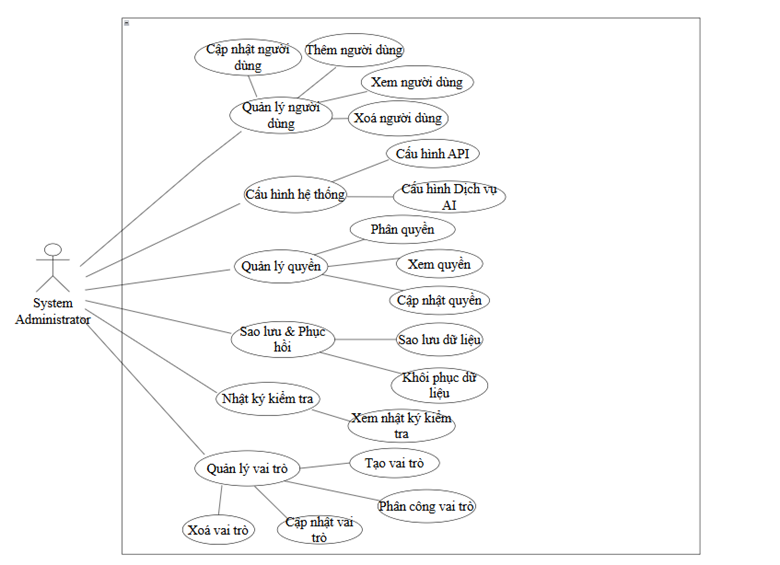
\includegraphics[width=6.5in,height=7.26597in,keepaspectratio,width=\linewidth]{images/Use case Diagram của Quản trị viên hệ thống.png}
\end{figure}

\textbf{Bảng mô tả các use case chính của Quản trị viên hệ thống}

% ==================== UC65 ====================
\begin{longtable}{|C{3cm}|L{11cm}|}
\hline
\textbf{Thành phần} & \textbf{Nội dung} \\
\hline
\textbf{Use Case ID} & UC65 \\
\hline
\textbf{Tên Use Case} & Quản lý người dùng \\
\hline
\textbf{Actor chính} & Quản trị viên hệ thống \\
\hline
\textbf{Mô tả} &
Cho phép quản trị viên quản lý tài khoản người dùng trong hệ thống.
\\
\hline
\textbf{Tiền điều kiện} &
Quản trị viên đã đăng nhập và có quyền quản lý người dùng.
\\
\hline
\textbf{Luồng chính} &
\begin{itemize}[leftmargin=*,topsep=2pt,itemsep=2pt]
    \item 1. Quản trị viên truy cập chức năng quản lý người dùng.
    \item 2. Hệ thống hiển thị danh sách người dùng.
    \item 3. Quản trị viên chọn người dùng cần thao tác.
    \item 4. Thực hiện xem, thêm, cập nhật hoặc vô hiệu hóa tài khoản.
    \item 5. Hệ thống kiểm tra dữ liệu.
    \item 6. Hệ thống lưu thay đổi và thông báo kết quả.
\end{itemize}
\\
\hline
\textbf{Luồng rẽ nhánh} &
\begin{itemize}[leftmargin=*,topsep=2pt,itemsep=2pt]
    \item 5a. Thông tin không hợp lệ $\rightarrow$ yêu cầu nhập lại.
    \item 5b. Tài khoản đã tồn tại $\rightarrow$ thông báo lỗi.
    \item 6a. Lưu thất bại $\rightarrow$ thông báo lỗi.
\end{itemize}
\\
\hline
\textbf{Hậu điều kiện} &
Thông tin người dùng được cập nhật theo thao tác của quản trị viên.
\\
\hline
\end{longtable}


% ==================== UC70 ====================
\begin{longtable}{|C{3cm}|L{11cm}|}
\hline
\textbf{Thành phần} & \textbf{Nội dung} \\
\hline
\textbf{Use Case ID} & UC70 \\
\hline
\textbf{Tên Use Case} & Quản lý vai trò \\
\hline
\textbf{Actor chính} & Quản trị viên hệ thống \\
\hline
\textbf{Mô tả} &
Cho phép quản trị viên tạo và quản lý các vai trò trong hệ thống.
\\
\hline
\textbf{Tiền điều kiện} &
Quản trị viên đã đăng nhập và có quyền quản lý vai trò.
\\
\hline
\textbf{Luồng chính} &
\begin{itemize}[leftmargin=*,topsep=2pt,itemsep=2pt]
    \item 1. Quản trị viên truy cập quản lý vai trò.
    \item 2. Hệ thống hiển thị danh sách vai trò.
    \item 3. Quản trị viên chọn tạo, cập nhật hoặc xóa vai trò.
    \item 4. Nhập hoặc chỉnh sửa thông tin vai trò.
    \item 5. Hệ thống kiểm tra dữ liệu.
    \item 6. Lưu thay đổi.
\end{itemize}
\\
\hline
\textbf{Luồng rẽ nhánh} &
\begin{itemize}[leftmargin=*,topsep=2pt,itemsep=2pt]
    \item 5a. Tên vai trò đã tồn tại $\rightarrow$ thông báo lỗi.
    \item 5b. Vai trò đang được sử dụng $\rightarrow$ không cho phép xóa.
\end{itemize}
\\
\hline
\textbf{Hậu điều kiện} &
Danh sách vai trò được cập nhật.
\\
\hline
\end{longtable}


% ==================== UC75 ====================
\begin{longtable}{|C{3cm}|L{11cm}|}
\hline
\textbf{Thành phần} & \textbf{Nội dung} \\
\hline
\textbf{Use Case ID} & UC75 \\
\hline
\textbf{Tên Use Case} & Quản lý quyền \\
\hline
\textbf{Actor chính} & Quản trị viên hệ thống \\
\hline
\textbf{Mô tả} &
Cho phép quản trị viên quản lý quyền truy cập và chức năng của các vai trò.
\\
\hline
\textbf{Tiền điều kiện} &
Quản trị viên đã đăng nhập. Các vai trò đã được tạo.
\\
\hline
\textbf{Luồng chính} &
\begin{itemize}[leftmargin=*,topsep=2pt,itemsep=2pt]
    \item 1. Quản trị viên mở chức năng quản lý quyền.
    \item 2. Hệ thống hiển thị danh sách vai trò và quyền.
    \item 3. Quản trị viên chọn vai trò.
    \item 4. Chọn các quyền cần cấp hoặc thu hồi.
    \item 5. Hệ thống kiểm tra quyền.
    \item 6. Lưu cấu hình phân quyền.
\end{itemize}
\\
\hline
\textbf{Luồng rẽ nhánh} &
\begin{itemize}[leftmargin=*,topsep=2pt,itemsep=2pt]
    \item 5a. Quyền không hợp lệ $\rightarrow$ từ chối thao tác.
    \item 6a. Cập nhật thất bại $\rightarrow$ thông báo lỗi.
\end{itemize}
\\
\hline
\textbf{Hậu điều kiện} &
Quyền truy cập của vai trò được cập nhật.
\\
\hline
\end{longtable}


% ==================== UC79 ====================
\begin{longtable}{|C{3cm}|L{11cm}|}
\hline
\textbf{Thành phần} & \textbf{Nội dung} \\
\hline
\textbf{Use Case ID} & UC79 \\
\hline
\textbf{Tên Use Case} & Cấu hình hệ thống \\
\hline
\textbf{Actor chính} & Quản trị viên hệ thống \\
\hline
\textbf{Mô tả} &
Cho phép quản trị viên cấu hình các thiết lập chung, API, thông báo và dịch vụ AI.
\\
\hline
\textbf{Tiền điều kiện} &
Quản trị viên đã đăng nhập và có quyền cấu hình hệ thống.
\\
\hline
\textbf{Luồng chính} &
\begin{itemize}[leftmargin=*,topsep=2pt,itemsep=2pt]
    \item 1. Quản trị viên truy cập cấu hình hệ thống.
    \item 2. Hệ thống hiển thị các nhóm cấu hình.
    \item 3. Quản trị viên chọn cấu hình cần thay đổi.
    \item 4. Nhập giá trị mới.
    \item 5. Hệ thống kiểm tra giá trị.
    \item 6. Lưu cấu hình.
    \item 7. Hệ thống áp dụng cấu hình mới.
\end{itemize}
\\
\hline
\textbf{Luồng rẽ nhánh} &
\begin{itemize}[leftmargin=*,topsep=2pt,itemsep=2pt]
    \item 5a. Giá trị không hợp lệ $\rightarrow$ yêu cầu nhập lại.
    \item 6a. Không thể lưu cấu hình $\rightarrow$ thông báo lỗi.
\end{itemize}
\\
\hline
\textbf{Hậu điều kiện} &
Cấu hình hệ thống được cập nhật.
\\
\hline
\end{longtable}


% ==================== UC80 ====================
\begin{longtable}{|C{3cm}|L{11cm}|}
\hline
\textbf{Thành phần} & \textbf{Nội dung} \\
\hline
\textbf{Use Case ID} & UC80 \\
\hline
\textbf{Tên Use Case} & Nhật ký kiểm tra \\
\hline
\textbf{Actor chính} & Quản trị viên hệ thống \\
\hline
\textbf{Mô tả} &
Cho phép quản trị viên giám sát các hoạt động quan trọng của hệ thống và người dùng thông qua nhật ký.
\\
\hline
\textbf{Tiền điều kiện} &
Quản trị viên đã đăng nhập và hệ thống có dữ liệu nhật ký.
\\
\hline
\textbf{Luồng chính} &
\begin{itemize}[leftmargin=*,topsep=2pt,itemsep=2pt]
    \item 1. Quản trị viên mở chức năng nhật ký.
    \item 2. Hệ thống truy vấn các bản ghi hoạt động.
    \item 3. Quản trị viên lọc theo người dùng, thời gian hoặc loại hoạt động.
    \item 4. Hệ thống hiển thị kết quả.
    \item 5. Quản trị viên xem chi tiết bản ghi.
\end{itemize}
\\
\hline
\textbf{Luồng rẽ nhánh} &
\begin{itemize}[leftmargin=*,topsep=2pt,itemsep=2pt]
    \item 2a. Không có nhật ký phù hợp $\rightarrow$ hiển thị thông báo.
    \item 2b. Không thể truy xuất dữ liệu $\rightarrow$ thông báo lỗi.
\end{itemize}
\\
\hline
\textbf{Hậu điều kiện} &
Nhật ký hoạt động được hiển thị để phục vụ kiểm tra và truy vết.
\\
\hline
\end{longtable}


% ==================== UC82 ====================
\begin{longtable}{|C{3cm}|L{11cm}|}
\hline
\textbf{Thành phần} & \textbf{Nội dung} \\
\hline
\textbf{Use Case ID} & UC82 \\
\hline
\textbf{Tên Use Case} & Sao lưu \& khôi phục \\
\hline
\textbf{Actor chính} & Quản trị viên hệ thống \\
\hline
\textbf{Mô tả} &
Cho phép quản trị viên thực hiện và quản lý việc sao lưu, khôi phục dữ liệu hệ thống.
\\
\hline
\textbf{Tiền điều kiện} &
Quản trị viên đã đăng nhập và có quyền quản trị dữ liệu.
\\
\hline
\textbf{Luồng chính} &
\begin{itemize}[leftmargin=*,topsep=2pt,itemsep=2pt]
    \item 1. Quản trị viên truy cập chức năng sao lưu \& khôi phục.
    \item 2. Chọn thao tác sao lưu hoặc khôi phục.
    \item 3. Hệ thống kiểm tra trạng thái cơ sở dữ liệu.
    \item 4. Thực hiện thao tác được yêu cầu.
    \item 5. Hệ thống ghi nhận kết quả.
    \item 6. Thông báo hoàn tất cho quản trị viên.
\end{itemize}
\\
\hline
\textbf{Luồng rẽ nhánh} &
\begin{itemize}[leftmargin=*,topsep=2pt,itemsep=2pt]
    \item 3a. Cơ sở dữ liệu không khả dụng $\rightarrow$ không thể thực hiện thao tác.
    \item 4a. Sao lưu/khôi phục thất bại $\rightarrow$ thông báo lỗi và ghi nhật ký.
\end{itemize}
\\
\hline
\textbf{Hậu điều kiện} &
Dữ liệu được sao lưu hoặc khôi phục thành công.
\\
\hline
\end{longtable}

